\chapter{라그랑지안, 장, 국소 입자 과정}

보손 장, 페르미온 장, 전자기장은 모두 파동과 같은 방정식을 따릅니다. 이 방정식에는 장 자체와 그 시간 및 공간 미분이 함께 들어갑니다. 각 장마다 운동 방정식을 하나씩 따로 나열할 수도 있지만, 라그랑지안은 전체 계를 하나의 간결한 식으로 모아 줍니다. 그 식에 오일러--라그랑주 규칙을 적용하면 모든 장의 방정식을 한꺼번에 얻습니다.

이 구성은 정지 작용 원리와 밀접하게 관련되어 있습니다. 여기서 당장 할 일은 더 구체적입니다. 장 라그랑지안이 어떤 양에 의존하는지 확인하고, 이를 이용해 몇 가지 고전 방정식을 얻은 다음, 같은 장의 식을 양자역학적으로 다시 해석하는 것입니다. 양자 이론에서 라그랑지안은 입자의 운동과 상호작용을 지배하며, 궁극적으로 충돌의 진폭과 단면적을 결정합니다.

\section{장 방정식을 간결하게 표현하는 방법}

하나의 스칼라 장에 대해 라그랑지안 밀도는 장과 그 1계 미분에 의존합니다.
\begin{equation}
\mathcal L
=
\mathcal L\!\left(\phi,\partial_t\phi,\partial_x\phi,\ldots\right)
=
\mathcal L\!\left(\phi,\partial_\mu\phi\right).
\end{equation}
계산할 때는 시간 및 공간 미분을 명시적으로 나열하는 편이 더 유용할 때가 많습니다. \(\partial_\mu\phi\) 표기는 같은 미분 목록을 상대론적 형태로 묶어 나타냅니다.

\begin{figure}[htbp]
\centering
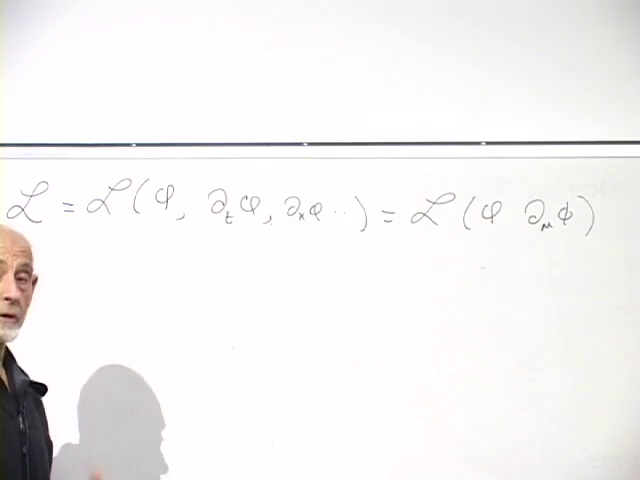
\includegraphics[width=0.82\textwidth]{lecture_09_figure_03.png}
\caption{스칼라 장의 라그랑지안이 장과 시공간 미분에 의존하는 모습.}
\lectureframe{00:03:56}
\end{figure}

장에 대한 오일러--라그랑주 방정식은 다음과 같습니다.
\begin{equation}
\frac{\partial}{\partial t}
\frac{\partial\mathcal L}{\partial\dot\phi}
+
\frac{\partial}{\partial x}
\frac{\partial\mathcal L}{\partial\phi_x}
+
\frac{\partial}{\partial y}
\frac{\partial\mathcal L}{\partial\phi_y}
+
\frac{\partial}{\partial z}
\frac{\partial\mathcal L}{\partial\phi_z}
=
\frac{\partial\mathcal L}{\partial\phi},
\end{equation}
여기서
\begin{equation}
\dot\phi=\frac{\partial\phi}{\partial t},
\qquad
\phi_x=\frac{\partial\phi}{\partial x},
\qquad
\phi_y=\frac{\partial\phi}{\partial y},
\qquad
\phi_z=\frac{\partial\phi}{\partial z}.
\end{equation}
\(\mathcal L\)에 여러 장이 들어 있으면 이 규칙을 각 장에 한 번씩 적용합니다. 그 결과 운동 방정식들의 계를 얻습니다.

가장 간단한 스칼라 예는 다음과 같습니다.
\begin{equation}
\begin{split}
\mathcal L
&=
\frac12\dot\phi^2
-\frac12\phi_x^2
-\frac12\phi_y^2
-\frac12\phi_z^2
-V(\phi)
\\
&=
\frac12\dot\phi^2-\frac12(\boldsymbol\nabla\phi)^2-V(\phi).
\end{split}
\end{equation}
공간 미분 항은 시간 미분 항과 부호가 반대입니다. 각 항을 미분하면
\begin{align}
\frac{\partial\mathcal L}{\partial\dot\phi}&=\dot\phi,
&
\frac{\partial\mathcal L}{\partial\phi_i}&=-\phi_i,
&
\frac{\partial\mathcal L}{\partial\phi}&=-V'(\phi),
\end{align}
따라서
\begin{equation}
\ddot\phi-\nabla^2\phi=-V'(\phi).
\end{equation}

\begin{figure}[htbp]
\centering
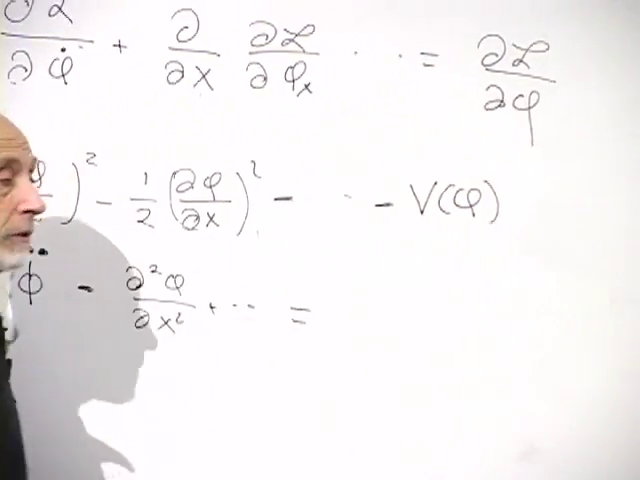
\includegraphics[width=0.74\textwidth]{lecture_09_figure_04.png}
\caption{오일러--라그랑주 방정식, 스칼라 장 라그랑지안, 그리고 \(V(\phi)\)가 만들어 내는 장 방정식.}
\lectureframe{00:08:23}
\end{figure}

이는 스칼라 라그랑지안이 만들어 내는 방정식입니다.\editorialnote{남아 있는 프레임은 왼쪽 가장자리가 잘려 있습니다. 화면에 보이는 완성된 식은 바로 앞뒤의 구술 유도에 따라 정해집니다.}

여기서 \(V(\phi)\)는 장의 퍼텐셜 에너지 밀도이다. \(V\)에 상수항을 더해도 미분하면 사라지므로 이 방정식에는 영향을 주지 않는다. 선형 퍼텐셜도 대수적으로는 가능하지만, 아래쪽 경계가 없다. 즉 장의 에너지는 음의 무한대로 내려갈 수 있다. 따라서 가장 단순한 안정적인 예는
\begin{equation}
V(\phi)=\frac12m^2\phi^2,
\qquad
V'(\phi)=m^2\phi,
\end{equation}
이며, 이로부터 다음을 얻는다.
\begin{equation}
\ddot\phi-\nabla^2\phi=-m^2\phi.
\end{equation}

\(m\)의 의미를 드러내기 위해 평면파를 대입합니다.
\begin{equation}
\phi(\mathbf x,t)=\phi_0e^{i\omega t-i\mathbf k\cdot\mathbf x}.
\end{equation}
그러면
\begin{equation}
\ddot\phi=-\omega^2\phi,
\qquad
\nabla^2\phi=-\mathbf k^2\phi,
\end{equation}
따라서 파동 방정식은 다음과 같이 됩니다.
\begin{equation}
-\omega^2\phi+\mathbf k^2\phi=-m^2\phi.
\end{equation}
\(\phi\)를 약분하면
\begin{equation}
\omega^2=\mathbf k^2+m^2.
\end{equation}
\(\hbar=c=1\)인 단위계에서는 진동수가 에너지이고 파수가 운동량입니다. 따라서
\begin{equation}
E^2=\mathbf p^2+m^2,
\end{equation}
또는 \(c\)의 거듭제곱을 복원하면 \(E^2=\mathbf p^2c^2+m^2c^4\)입니다. 매개변수 \(m\)는 이 장의 양자 하나의 질량입니다.

상대론적 불변성은 간결한 식의 수준에서 부과할 수 있습니다. \(\mathcal L\)가 로런츠 스칼라라면 그 운동 방정식은 로런츠 불변입니다. 시간 미분과 공간 미분 사이의 상대적 부호는 특수 상대론에서 익숙한 시공간 부호입니다.

\section{비선형성과 결합된 고전장}

장에 더 높은 거듭제곱을 포함하면 새로운 종류의 거동이 나타납니다. 만약
\begin{equation}
V(\phi)=\frac12m^2\phi^2+g\phi^3,
\end{equation}
이라면
\begin{equation}
\ddot\phi-\nabla^2\phi=-m^2\phi-3g\phi^2.
\end{equation}
라그랑지안의 이차항은 장에 대해 선형인 방정식을 만듭니다. 삼차항과 그보다 높은 항은 비선형 방정식을 만듭니다.

이 차이는 파동 묶음의 운동에서 드러납니다. 선형 방정식에서는 오른쪽으로 움직이는 파동 묶음과 왼쪽으로 움직이는 파동 묶음을 더해 또 다른 해를 만들 수 있습니다. 두 묶음은 잠시 겹쳐 간섭한 다음 서로 통과해 지나가며 원래 형태로 나타납니다. 비선형 항이 있으면 파동 묶음은 서로에게 영향을 줍니다. 서로 산란하거나 변형되거나 더 복잡한 파동으로 분해될 수 있습니다. 선형파의 일시적인 간섭은 상호작용이 아닙니다. 파동 묶음에 지속적인 변화가 생긴다면 이는 비선형성을 나타냅니다.

두 스칼라 장에서도 같은 양상이 나타납니다. 다음과 같이 두겠습니다.
\begin{align}
\mathcal L
&=
\frac12(\partial_\mu\phi)(\partial^\mu\phi)
+\frac12(\partial_\mu\rho)(\partial^\mu\rho)
-V(\phi,\rho),
\\
V(\phi,\rho)
&=
\frac12m^2\phi^2+\frac12M^2\rho^2+\rho\phi^2.
\end{align}
마지막 항이 없으면 두 방정식은 서로 독립입니다.
\begin{equation}
\ddot\phi-\nabla^2\phi=-m^2\phi,
\qquad
\ddot\rho-\nabla^2\rho=-M^2\rho.
\end{equation}
이 방정식들은 질량이 \(m\)와 \(M\)인 두 종류의 입자 양자를 나타냅니다. 혼합항을 포함하면
\begin{align}
\ddot\phi-\nabla^2\phi&=-m^2\phi-2\rho\phi,
\\
\ddot\rho-\nabla^2\rho&=-M^2\rho-\phi^2.
\end{align}
각 방정식에 이제 다른 장이 들어갑니다. 두 방정식은 결합되어 있고 비선형입니다. \(\phi\) 파동 묶음은 \(\rho\) 파동 묶음을 산란시키며, 그 반대도 마찬가지입니다. 미분항은 에너지--운동량 관계를 결정하고, 미분되지 않은 이차항은 질량을 정하며, 혼합된 고차항은 상호작용을 나타냅니다. 이것이 기본적인 고전적 양상입니다.

\section{디랙 장과 스칼라 결합}

디랙 장의 방정식은 시간에 대해 1계입니다. 세 공간 방향으로 확장할 수 있음을 전제로 1차원 표기로 쓰면 항의 구조는 다음과 같습니다.
\begin{equation}
i\dot\Psi
\simeq
i\alpha\frac{\partial\Psi}{\partial x}+m\beta\Psi,
\qquad
i\boldsymbol\alpha\cdot\boldsymbol\nabla\Psi
=i\sum_i\alpha_i\frac{\partial\Psi}{\partial x_i}.
\end{equation}
행렬 \(\alpha_i\)와 \(\beta\)는 \(\Psi\)의 성분에 작용합니다. 이에 대응하는 라그랑지안에는 \(\partial_t\Psi\)에 선형인 항, \(\alpha_i\)가 포함된 공간 미분 쌍선형항, 그리고 질량 쌍선형항 \(m\Psi^\dagger\beta\Psi\)이 들어갑니다. 여기서는 이 구조적 사실만 알면 충분합니다.\editorialnote{출처에서 시도한 디랙 라그랑지안의 부호, 괄호, 그리고 \(i\)의 위치는 명시적으로 미정으로 남아 있습니다. 이로부터 관례에 따라 달라지는 정확한 식을 추론하지 않습니다.}

\begin{figure}[htbp]
\centering
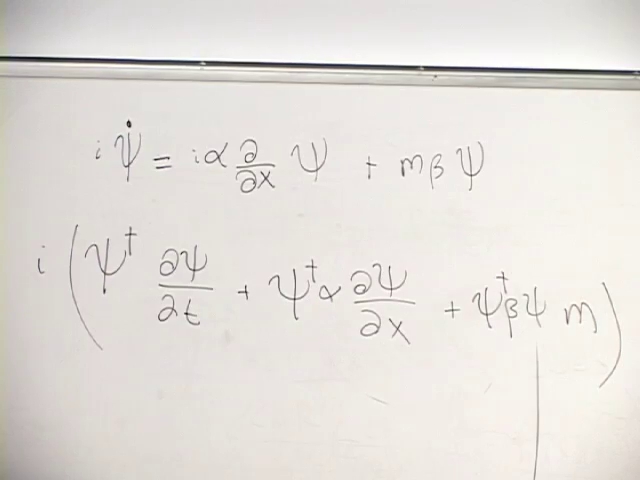
\includegraphics[width=0.76\textwidth]{lecture_09_figure_05.png}
\caption{디랙 장 논의에서의 시간 미분항, 공간 미분항, 질량항.}
\lectureframe{00:25:37}
\end{figure}

\begin{classroomqa}
\lecturetimestamp{00:26:37}
\audiencequestion{시도된 디랙 라그랑지안에서 괄호의 위치는 올바른가요? \(i\)가 전체 식에 곱해지는 건가요?}
\lecturerresponse{여기서는 그 위치를 확신을 가지고 정하지 않으며, 구조적 요점을 위해 꼭 필요한 것도 아닙니다. 디랙 방정식을 만들어 내는 라그랑지안이 존재합니다.}
\end{classroomqa}

이제 스칼라 장 \(\phi\)를 더해 보겠습니다. 단순한 곱 \(\Psi^\dagger\Psi\,\phi\)는 로런츠 스칼라가 아닙니다. 질량항에 나타나는 것과 같은 디랙 행렬을 넣으면
\begin{equation}
\mathcal L_{\mathrm{int}}
\propto
\Psi^\dagger\beta\Psi\,\phi.
\end{equation}
같은 뜻으로 \(\Psi^\dagger\beta\Psi\)는 스칼라 디랙 쌍선형입니다. 전체 라그랑지안을 변분하면 디랙 방정식에는 \(\phi\)에 비례하는 항이 더해지고, 스칼라 방정식에는 \(\Psi^\dagger\beta\Psi\)에 비례하는 원천항이 더해집니다. 두 장은 서로를 산란시킵니다.

\begin{classroomqa}
\lecturetimestamp{00:28:03}
\audiencequestion{스칼라--페르미온 상호작용에 넣은 \(\beta\)는 디랙 질량항에 나타나는 것과 같은 \(\beta\)인가요?}
\lecturerresponse{네. 같은 디랙 행렬입니다.}
\end{classroomqa}

비교식
\begin{equation}
m\Psi^\dagger\beta\Psi
\qquad\hbox{and}\qquad
\Psi^\dagger\beta\Psi\,\phi
\end{equation}
을 보면 결합항에서 질량 매개변수가 스칼라장으로 대체된 것처럼 보인다. 진공 기댓값이 영이 아닌 장을 끝부분에서 살펴볼 때 이 관찰을 다시 다룬다.

지금까지의 해석은 고전적이었습니다. 파동 묶음이 다른 파동 묶음을 산란시킵니다. 장이 연산자가 되면 같은 대수적 구조가 입자에 대해 더 명확한 의미를 갖습니다.

\section{양자장의 거듭제곱이 하는 일}

실수 스칼라 양자장은 생성 연산자와 소멸 연산자를 모두 포함합니다. 개략적으로 쓰면
\begin{equation}
\phi(x)\sim A^+(x)+A^-(x),
\end{equation}
여기서 \(A^+\)는 양자 하나를 생성하고 \(A^-\)는 하나를 소멸시킵니다. 따라서 \(\phi^3(x)\)에는 다음 네 종류의 국소 과정이 들어 있습니다.
\begin{equation}
\phi^3
\sim
(A^+)^3+(A^+)^2A^-+A^+(A^-)^2+(A^-)^3,
\end{equation}
이 개략적 해석에서는 연산자 순서의 세부 사항과 수치 계수를 생략했습니다. 입자 수의 변화는 다음 네 가지입니다.
\begin{equation}
3\longrightarrow0,
\qquad
0\longrightarrow3,
\qquad
2\longrightarrow1,
\qquad
1\longrightarrow2.
\end{equation}
세 장 인자는 모두 같은 점 \(x\)에서 작용합니다. 따라서 하나의 삼차항에는 입자 셋의 소멸, 입자 셋의 생성, 양자 둘이 하나로 합쳐지는 과정, 그리고 양자 하나가 둘로 분리되는 과정이 모두 들어 있습니다. 실제 진폭에서는 에너지--운동량 보존 때문에 이러한 국소적 해석 중 일부가 나중에 제외될 수 있지만, 연산자 곱 자체에는 모두 들어 있습니다.

이차 자유항은 역할이 다릅니다. 먼저 이웃한 점 \(x\)와 \(x'\) 사이의 차이에 붙는 정규화 계수를 잠시 생략하면
\begin{equation}
\partial_x\phi
\ \propto\
\phi(x)-\phi(x').
\end{equation}
제곱하여 전개하면 항의 구조는 다음과 같습니다.
\begin{align}
\frac12(\partial_x\phi)^2
&\ \propto\
\frac12\bigl[\phi(x)-\phi(x')\bigr]^2
\\
&=
\frac12\phi(x)^2
+\frac12\phi(x')^2
-\phi(x)\phi(x').
\end{align}
각 같은 점에서의 제곱에는 여러 연산자 해석이 있습니다. 양자 둘을 생성하거나 둘을 소멸할 수도 있고, 같은 점에서 양자 하나를 소멸시켰다가 다시 생성할 수도 있습니다. 이런 항은 입자를 다른 곳으로 옮기지 않습니다. 교차항은 \(x'\)에서 양자를 소멸시키고 \(x\)에서 생성하거나, 그 반대로 작용할 수 있습니다. 따라서 이 항은 가장 가까운 이웃 사이의 호핑 항으로 작용합니다. 이런 인자가 반복되면 입자가 \(x\)에서 \(x'\)로, 다시 \(x''\)로, 이어서 더 멀리 이동합니다. 이차 미분항은 자유 전파를 지배하고, 삼차항과 그보다 높은 항은 입자를 산란시키고 생성하며 소멸시킵니다.

\begin{classroomqa}
\lecturetimestamp{00:36:07}
\audiencequestion{유한 차분으로 미분을 나타낼 때 점 사이의 거리 \(x-x'\)도 포함해야 하나요?}
\lecturerresponse{그렇습니다. 거리를 \(L\)라고 하면 차분을 제곱한 뒤 인자 \(L^{-2}\)가 생깁니다. 이 수치 인자는 계수를 바꾸지만 호핑이라는 해석은 바꾸지 않습니다.}
\end{classroomqa}

거리를 복원하면
\begin{align}
\frac12(\partial_x\phi)^2
&\longrightarrow
\frac{1}{2L^2}\bigl[\phi(x)-\phi(x')\bigr]^2
\\
&=
\frac{1}{2L^2}\phi(x)^2
+\frac{1}{2L^2}\phi(x')^2
-\frac{1}{L^2}\phi(x)\phi(x').
\end{align}

질량항도 이차항이지만 미분은 포함하지 않습니다.
\begin{equation}
\frac12m^2\phi(x)^2.
\end{equation}
이 항을 입자 하나에 대해 해석하면 들어오는 양자가 같은 점에서 흡수되었다가 다시 방출됩니다. 양자를 이동시키지는 않습니다. 그 점에 양자가 존재하는 정도에 가중치를 주거나, 그런 의미에서 양자의 존재를 세는 항입니다. 같은 연산자 제곱에는 양자 둘을 생성하거나 소멸하는 해석도 포함됩니다. 따라서 운동과 관련해 중요한 차이는 이웃한 점들을 잇는 교차항과 한 점 안에서 작용하는 질량 삽입항 사이에 있습니다.

\section{양자전기역학의 국소 꼭짓점}

이런 기본적인 입자 과정의 개략도에서 파인만 도표가 시작됩니다. 핵심 예는 전자, 양전자, 광자의 이론인 양자전기역학입니다.

디랙 방정식에는 양의 에너지 모드와 음의 에너지 모드가 있습니다. 오래된 표현으로는 \(\Psi\)가 두 종류 모드의 소멸 연산자를 포함하고, \(\Psi^\dagger\)는 이에 대응하는 생성 연산자를 포함합니다. 음의 에너지 전자를 제거하는 것은 양의 에너지를 가진 양전자를 생성하는 것으로 재해석됩니다. 이렇게 표기를 바꾸면 유용한 개략적 분해는 다음과 같습니다.
\begin{align}
\Psi
&\sim
C^-_{e^-}+C^+_{e^+},
\\
\Psi^\dagger
&\sim
C^+_{e^-}+C^-_{e^+}.
\end{align}
따라서 \(\Psi\)는 전자를 소멸시키거나 양전자를 생성하고, \(\Psi^\dagger\)는 전자를 생성하거나 양전자를 소멸시킵니다. 이 약식 표기에는 정규화, 스핀 표지, 운동량 적분이 포함되어 있지 않습니다.

양자전기역학의 상호작용은 디랙 전류와 전자기 벡터 퍼텐셜을 결합합니다. 여기서 사용하는 성분 표기에서 그 구조는 다음과 같습니다.
\begin{equation}
\mathcal L_{\mathrm{QED,int}}
\sim
e\left(
\Psi^\dagger\Psi\,A_0
+
\Psi^\dagger\boldsymbol{\alpha}\Psi\mathbin{\boldsymbol{\cdot}}\mathbf A
\right),
\end{equation}
여기서
\begin{equation}
J^0=\Psi^\dagger\Psi,
\qquad
\mathbf J=\Psi^\dagger\boldsymbol{\alpha}\Psi.
\end{equation}
기호 \(\sim\)가 중요합니다. 시간 성분과 공간 성분 사이의 상대적 부호는 계량 부호 규약과 벡터 퍼텐셜의 규약에 따라 달라집니다. 불변인 진술은 4전류와 4퍼텐셜을 축약한다는 것입니다.\editorialnote{출처는 전류의 시간 성분과 공간 성분을 정하지만, 성분 축약에 적용할 계량 규약은 정하지 않습니다.}

광자장 \(A_\mu\) 자체에는 광자의 생성 및 소멸 연산자가 들어 있습니다. 벡터라는 성질에는 운동량뿐 아니라 광자의 편광---작은 방향 ``표지''도 담겨 있습니다.

\begin{classroomqa}
\lecturetimestamp{00:44:28}
\audiencequestion{\(A_\mu\)가 벡터이고 페르미온 인자는 처음 보면 스칼라 같은데, 상호작용은 어떻게 스칼라가 될 수 있나요?}
\lecturerresponse{페르미온도 4벡터를 제공합니다. \(\Psi^\dagger\Psi\)는 그 시간 성분이고 \(\Psi^\dagger\boldsymbol\alpha\Psi\)는 공간 성분입니다. 이 전류를 \(A_\mu\)와 축약하면 스칼라가 됩니다.}
\end{classroomqa}

\(\Psi^\dagger\), \(\Psi\), \(A_\mu\)의 연산자 내용을 곱하면 하나의 국소 꼭짓점에 대해 익숙한 네 가지 해석을 얻습니다.
\begin{enumerate}\item 전자가 광자를 방출한다;
\item 전자가 광자를 흡수한다;
\item 전자와 양전자가 소멸하여 광자가 된다;
\item 광자가 전자--양전자 쌍을 생성한다.
\end{enumerate}
첫 번째 해석에서 \(\Psi\)는 들어오는 전자를 소멸시키고, \(\Psi^\dagger\)는 나가는 전자를 생성하며, 광자장은 광자를 생성합니다. 광자장의 소멸 부분을 택하면 흡수가 됩니다. 양전자에 해당하는 부분을 택하면 쌍 소멸 또는 쌍 생성이 됩니다. 하나의 국소항에 이 과정들이 모두 들어 있습니다.

페르미온 흐름 도표에서 양전자 선의 화살표는 양전자의 전파 방향과 반대로 향합니다. 이 규약을 따르면 허용된 모든 양자전기역학 꼭짓점에서 페르미온 화살표가 끊기지 않고 이어집니다. 네 가지 해석은 외부 다리를 들어오는 쪽과 나가는 쪽 사이에서 옮겨서 구별할 뿐, 페르미온 흐름선을 끊지는 않습니다.

이 모든 해석에는 같은 계수 \(e\)가 붙습니다. 이는 여기서 사용하는 미시적 규약의 전하입니다. 이 계수는 미세구조상수가 아니라 전하 \(e\)이지만, 두 양은 밀접하게 관련되어 있습니다. 꼭짓점 진폭은 \(e\)에 비례하고, 모든 운동학적 인자와 정규화 인자를 포함하면 그에 대응하는 확률의 척도는 \(e^2\)에 비례합니다.

\begin{classroomqa}
\lecturetimestamp{00:49:44}
\audiencequestion{광자가 전자--양전자로 바뀌는 해석에도 꼭짓점의 다른 해석과 같은 계수가 붙나요?}
\lecturerresponse{네. 같은 전하 계수 \(e\)가 붙습니다.}
\end{classroomqa}

\begin{classroomqa}
\lecturetimestamp{00:49:59}
\audiencequestion{확률에는 단위가 없으니 어떤 스케일링 인자가 있어야 하지 않나요?}
\lecturerresponse{여기서 사용하는 자연스러운 미시적 규약에서 전하 \(e\)는 무차원입니다. 진폭의 척도는 전하이고, 그 제곱이 확률의 척도를 제공합니다.}
\end{classroomqa}

구체적인 그림으로, 전자가 벽에 부딪혀 갑자기 멈추는 상황을 생각해 봅시다. 에너지와 운동량이 광자 형태로 빠져나갈 확률이 있습니다. 그 복사 진폭에 들어가는 기본적인 전자기 인자는 \(e\)이므로 확률의 척도에는 \(e^2\)가 들어갑니다. 이 진술은 결합 인자만 따로 나타낸 것입니다. 실제 확률은 전자의 상태와 운동학에도 달려 있습니다.

\begin{figure}[htbp]
\centering
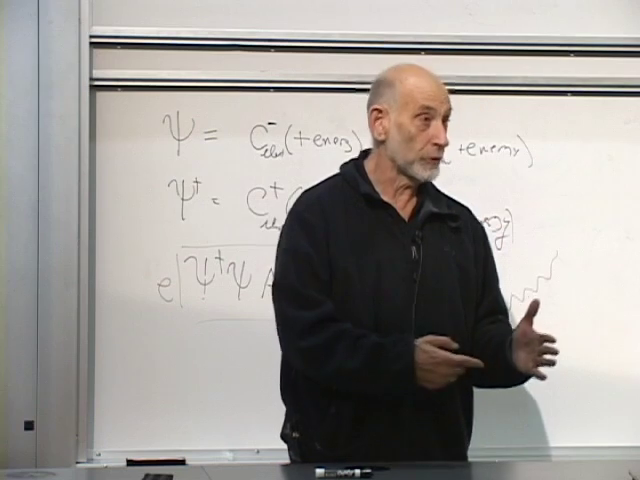
\includegraphics[width=0.78\textwidth]{lecture_09_figure_06.png}
\caption{\(\Psi\)와 \(\Psi^\dagger\)의 전자 및 양전자 연산자 내용과 전자--광자 상호작용 개략도.}
\lectureframe{00:50:39}
\end{figure}

\begin{classroomqa}
\lecturetimestamp{00:51:15}
\audiencequestion{전하에는 단위가 있나요?}
\lecturerresponse{여기서 사용하는 자연스러운 미시적 규약에서는 단위가 없습니다. 거시적 전하는 흔히 쿨롱으로 나타내지만, 입자 이론에서는 전하를 정해 둔 기본 단위를 기준으로 측정합니다. 플랑크 단위나 다른 자연 단위계에서는 물리량을 순수한 수로 나타냅니다.}
\end{classroomqa}

관례와 척도의 차이입니다. 전선의 전류를 다룰 때는 쿨롱이 편리하고, 미시적 진폭을 다룰 때는 무차원 결합이 편리합니다.\editorialnote{00에서 52:37--00:53:15에 나온 ``전하를 가진 항의 묶기''에 관한 짧은 질문은 상당 부분 손상되어 있어, 확정적인 구성을 이끌어 내지 못했습니다.}

기본적인 양자전기역학 상호작용에서 세 장은 모두 한 시공간 점에서 평가됩니다. 꼭짓점 자체에는 내부 시간 지연이 부여되지 않습니다.

\begin{classroomqa}
\lecturetimestamp{00:53:19}
\audiencequestion{전자의 흡수와 재방출, 그리고 광자의 방출은 동시에 일어나나요? 아니면 방정식에 지연이 들어 있나요?}
\lecturerresponse{기본 꼭짓점에서는 모든 연산자가 같은 시공간 점에서 평가됩니다. 따라서 기본 과정에서 이 작용들 사이에는 지연이 없습니다.}
\end{classroomqa}

\begin{classroomqa}
\lecturetimestamp{00:53:57}
\audiencequestion{보존되는 각 물리량은 서로 따로 보존되어야 하나요?}
\lecturerresponse{그렇습니다. 전하는 따로 보존되어야 하는 물리량 가운데 하나입니다.}
\end{classroomqa}

전하 보존은 도표와 대수 양쪽에서 확인할 수 있습니다. 들어오는 전자가 나가는 양전자로 바뀌는 과정은 전하의 부호를 뒤집으므로 허용되는 양자전기역학 꼭짓점이 아닙니다. 시간을 위쪽으로 그리면 전자의 화살표는 시간 방향을 따라 위로 향하고 양전자의 화살표는 아래로 향합니다. 유효한 꼭짓점에서는 페르미온 화살표가 항상 이어집니다. 대수적으로 상호작용에는 \(\Psi\) 하나와 \(\Psi^\dagger\) 하나가 들어 있습니다. 첫 번째 연산자는 전자를 소멸시키거나 양전자를 생성할 때 전하를 한 단위만큼 높이고, 두 번째 연산자는 전하를 한 단위만큼 낮춥니다. 두 효과는 서로 상쇄됩니다.

\begin{classroomqa}
\lecturetimestamp{00:56:05}
\audiencequestion{상자 안의 전자--광자 식이 양자전기역학 라그랑지안 전체인가요?}
\lecturerresponse{아닙니다. 이것은 상호작용항입니다. 전파를 지배하는 이차 자유 광자항과 이차 디랙항은 쓰지 않았습니다.}
\end{classroomqa}

\begin{classroomqa}
\lecturetimestamp{00:56:35}
\audiencequestion{고전 라그랑지안은 유도하고 양자 라그랑지안은 추측한 뒤 검증하나요? 그리고 운동에너지에서 퍼텐셜 에너지를 뺀 구조는 양자역학에서도 유지되나요?}
\lecturerresponse{운동에너지에서 퍼텐셜 에너지를 빼는 양상은 유지됩니다. 시간 미분은 운동에너지 형태를 제공하고, 공간 기울기는 이를 일반화하며, 미분되지 않은 장 항은 퍼텐셜 에너지 형태를 제공합니다. 양자 라그랑지안이 더 근본적인 기술입니다. 양자가 매우 많이 들어 있는 상태에서는 같은 라그랑지안이 고전적인 파동 방정식을 만들어 냅니다. 후보 라그랑지안은 물리 원리와 더 깊은 이론을 바탕으로 제안한 뒤 충돌 실험으로 확립하거나 배제합니다.}
\end{classroomqa}

점유수가 큰 극한은 같은 식이 양자 입자 이론과 그 고전적인 파동을 모두 지배할 수 있는 이유를 설명합니다. 이 일치는 나중에 별도의 기적처럼 덧붙이는 것이 아닙니다. 고전장은 많은 양자가 집단적으로 보이는 거동입니다. 반대로 충돌 실험에서는 기본 꼭짓점이 직접 드러나므로 양자전기역학과 표준 모형의 상호작용을 매우 정밀하게 결정할 수 있습니다.

\section{교차와 시공간 보존 법칙}

국소 꼭짓점의 다리는 들어오는 위치와 나가는 위치 사이에서 교차해 옮겨질 수 있습니다. 나가는 입자를 들어오는 쪽으로 옮기면 그 입자는 반입자로 재해석되며, 반대도 마찬가지입니다. 이런 의미에서 같은 전자--양전자--광자 연산자는 방출, 흡수, 쌍 소멸, 쌍 생성, 심지어 모두 들어오는 국소 해석까지 나타낼 수 있습니다.

\begin{classroomqa}
\lecturetimestamp{00:59:34}
\audiencequestion{기본 꼭짓점 도표를 회전하면 여전히 유효한 국소 해석인가요?}
\lecturerresponse{그렇습니다. 외부 다리를 들어오는 위치와 나가는 위치 사이에서 옮기면 그에 따라 입자--반입자로 재해석할 수 있습니다.}
\end{classroomqa}

국소 연산자 관점만으로는 물리적 과정이 완전히 기술되지 않는다. 꼭짓점이 생길 수 있는 모든 시공간 지점에 대해 진폭을 적분해야 한다. 시간 적분은 에너지 보존을, 공간 적분은 운동량 보존을 보장한다. 전자와 양전자, 광자가 모두 진공 속으로 사라지는 그림은 형식적인 국소 관점으로는 성립하지만, 이 과정은 에너지와 운동량을 보존할 수 없으므로 적분한 진폭은 영이 된다.

\begin{classroomqa}
\lecturetimestamp{01:00:30}
\audiencequestion{모두 들어오는 그림은 전자, 양전자, 광자가 아무것도 남기지 않고 사라질 수 있다는 뜻인가요?}
\lecturerresponse{이는 국소 연산자의 한 해석이지만, 물리적 진폭에는 꼭짓점 위치에 대한 적분이 포함됩니다. 이 적분들은 에너지와 운동량 보존을 강제하므로 운동학적으로 금지된 이 과정의 진폭은 0입니다.}
\end{classroomqa}

\begin{classroomqa}
\lecturetimestamp{01:01:57}
\audiencequestion{그 반대인 진공에서 전자--양전자--광자가 생성되는 해석도 있나요? 배제되는 과정은 적분 뒤에 사라지나요?}
\lecturerresponse{그 반대의 국소 해석도 들어 있습니다. 공간과 시간에 대한 적분은 보존 법칙에 맞지 않는 모든 과정을 제거합니다.}
\end{classroomqa}

라그랑지안의 미분은 생성 및 소멸 기호 자체를 미분하지 않아도 연산자 전개와 잘 맞습니다. 장의 개략적 형태는 다음과 같습니다.
\begin{equation}
\Psi(x)
\sim
\int d^3k\,
\bigl[
C(\mathbf k)e^{i\mathbf k\cdot\mathbf x-i\omega t}
+\cdots
\bigr].
\end{equation}
연산자 \(C(\mathbf k)\)는 이 시공간 전개의 계수입니다. 미분은 평면파에 작용하여 \(\mathbf k\) 또는 \(\omega\)를 끌어냅니다.

\begin{classroomqa}
\lecturetimestamp{01:02:27}
\audiencequestion{장 전개식을 미분할 때 생성 연산자 자체도 미분하나요?}
\lecturerresponse{아닙니다. 이 전개에서 생성 연산자와 소멸 연산자는 시공간 좌표에 의존하지 않습니다. 미분은 지수 인자에 작용해 운동량과 진동수를 끌어냅니다.}
\end{classroomqa}

\section{유효 이론으로서의 핵자와 파이온}

같은 표현법으로 양성자, 중성자, 파이온을 기술할 수 있습니다. 양성자와 중성자는 \(\Psi_p\)와 \(\Psi_n\)라는 장으로 나타내는 페르미온입니다. 상호작용을 세는 이 논의에서는 파이온 장을 세 가지 전하 상태를 갖는 스칼라 장으로 취급합니다.
\begin{equation}
\pi^+,
\qquad
\pi^-,
\qquad
\pi^0.
\end{equation}
양성자와 \(\pi^+\)는 전하를 한 단위만큼 띠고, \(\pi^-\)는 음전하를 한 단위만큼 띠며, 중성자와 \(\pi^0\)는 중성입니다. 더 깊은 수준에서 파이온은 쿼크--반쿼크 계이지만, 처음에는 그 내부 구조를 미정으로 두어도 됩니다.

전하를 보존하는 핵자--파이온 장 곱의 개략적인 목록은 다음과 같습니다.
\begin{equation}
\mathcal L_{N\pi}
\sim
\left\{
\Psi_p^\dagger\Psi_n\,\pi^+,\;
\Psi_n^\dagger\Psi_p\,\pi^-,\;
\Psi_p^\dagger\Psi_p\,\pi^0,\;
\Psi_n^\dagger\Psi_n\,\pi^0
\right\}.
\end{equation}
여기서는 장의 구성과 전하 배정만 나타냅니다. 상대 계수와 부호, 스피너 행렬 구조는 정해져 있지 않습니다. 첫 번째 파이온 장의 전하는 구체적인 해석을 따져 확인할 수 있습니다. 중성자와 양전하 파이온 하나는 양성자를 만들 수 있지만, 그 자리에 음전하 파이온을 쓰면 들어오는 음전하가 나가는 양전하로 바뀝니다. 켤레항은 반대 전하를 띤 과정을 나타냅니다.\editorialnote{출처에서는 전하를 보존하는 한 쌍의 항에 도달하기 전까지 파이온 부호를 여러 차례 수정합니다. 표시된 순서는 최종적인 개략 구조를 반영합니다.}

각 항은 다시 여러 방식으로 교차 해석할 수 있습니다. 나가는 중성자를 들어오는 쪽으로 옮기면 들어오는 반중성자로 바뀝니다. 따라서 전하를 띤 꼭짓점은 양성자와 반중성자가 결합해 \(\pi^+\)가 되는 과정을 나타낼 수 있고, 운동학적으로 가능하면 \(p\to n+\pi^+\) 같은 과정도 나타낼 수 있습니다. 중성 항은 양성자나 중성자가 \(\pi^0\)를 방출하거나 흡수하도록 합니다. 전하 보존은 허용되는 과정의 종류를 정하고, 에너지와 운동량 및 그 밖의 대칭성은 특정 실험에서 그중 어떤 과정이 일어날 수 있는지를 결정합니다.

쿼크 내부 구조가 알려지기 전에는 이것이 유용한 유효 기술이었습니다. 탐침으로 그 구조를 분해해 볼 수 없을 때는 지금도 유용합니다. 양성자에는 원자에 내부 구조가 있는 것처럼 유한한 분포를 가진 구성 입자들이 있지만, 그 규모는 훨씬 작습니다. 실험에서 전달하는 운동량이 양성자를 분해하거나 그 구조를 알아볼 만큼 크지 않다면 양성자를 고유한 장을 가진 점입자로 취급할 수 있습니다. 충분히 높은 에너지의 충돌은 쿼크를 드러내므로, 그때는 점입자로서의 양성자 장만으로는 더 이상 충분하지 않습니다.

양성자는 전하를 띠므로 국소적인 양성자--광자 상호작용도 있습니다. 개략적으로는 \(J_p^\mu A_\mu\)이며, 여기서 \(J_p^\mu\)는 양성자 전류입니다. 전자에도 이에 대응하는 전자--광자 상호작용이 있습니다. 양성자는 광자를 방출하면서 중성자로 바뀔 수는 없습니다. \(p\to n+\gamma\)는 전하 보존을 위반합니다.

\begin{classroomqa}
\lecturetimestamp{01:10:28}
\audiencequestion{양성자와 전자가 상호작용하면 어떻게 되나요?}
\lecturerresponse{각 전하 입자에는 광자 꼭짓점이 있습니다. 양성자는 양성자로 남은 채 광자를 방출할 수 있고, 전자는 전자로 남은 채 그 광자를 흡수할 수 있습니다. 양성자--전자 산란은 이 두 국소 꼭짓점과 그 사이에서 전파되는 광자로 이루어집니다.}
\end{classroomqa}

\section{국소성과 기본 과정의 반복}

양성자--전자 사이의 전체 교환을 나타내는 특별한 비국소 항은 없습니다. 하나의 국소 꼭짓점에서 양성자가 광자를 방출하고, 이차 광자항들이 이웃한 점에서 다음 이웃한 점으로 광자를 전달하며, 또 다른 국소 꼭짓점에서 전자가 이를 흡수합니다. 확장된 과정은 이러한 기본 조각들을 곱해 얻습니다.
\begin{equation}
\begin{aligned}
\bigl[J_p^\mu A_\mu\bigr](x_p)
&\longrightarrow
\underbrace{x_p\to x_1\to x_2\to\cdots\to x_e}_{\text{quadratic photon propagation}}
\\
&\longrightarrow
\bigl[J_e^\nu A_\nu\bigr](x_e).
\end{aligned}
\end{equation}
이 개략적인 연쇄의 화살표는 연이어 일어나는 이웃 점 삽입을 나타내며, 새로운 비국소 상호작용을 뜻하지 않습니다.

\begin{classroomqa}
\lecturetimestamp{01:12:06}
\audiencequestion{양성자와 전자가 서로 교환되는 전체 과정의 라그랑지안은 어떻게 쓸까요--?}
\lecturerresponse{이렇게 전체에 걸친 사건을 나타내는 항을 따로 더하지는 않습니다. 이 과정은 국소적인 양성자--광자 꼭짓점, 반복되는 이차 전파 항, 국소적인 전자--광자 꼭짓점으로 이루어집니다.}
\end{classroomqa}

국소 구조는 두 가지 형태를 가집니다. 미분되지 않은 상호작용 항은 하나의 시공간 점에서 작용합니다. 유한 차분으로 표현되는 미분 항은 그 점을 이웃한 점과만 연결합니다. 어느 형태도 입자를 유한한 거리에 걸쳐 직접 옮기지 않습니다. 장거리 전파는 무수히 많은 무한소 이동을 모아 이루어지며, 기본적인 원격 작용은 없습니다.

\begin{classroomqa}
\lecturetimestamp{01:14:36}
\audiencequestion{라그랑지안에는 한 점에서만 작용하는 항이 들어 있나요?}
\lecturerresponse{상호작용 항은 한 점에서 작용합니다. 미분 항은 한 점과 무한소만큼 이웃한 점을 연결합니다. 방출, 여러 차례의 이웃한 점 사이 이동, 흡수가 함께 유한한 교환을 만들어 냅니다.}
\end{classroomqa}

\begin{classroomqa}
\lecturetimestamp{01:15:36}
\audiencequestion{확장된 과정의 모든 요소가 들어 있나요? 그리고 이 요소들을 결합한다는 것은 곱한다는 뜻인가요?}
\lecturerresponse{그렇습니다. 기본적인 방출, 이동, 흡수는 각각 라그랑지안에 부호화되어 있습니다. 반복 삽입의 곱이 이 요소들을 결합해 더 큰 과정을 이룹니다.}
\end{classroomqa}

여기서 다루는 상대론적 양자장론은 장이 정의되는 시공간을 전제로 합니다. 이를 동역학적 시공간 기하학의 완전한 양자 이론과 혼동해서는 안 됩니다.

\begin{classroomqa}
\lecturetimestamp{01:16:28}
\audiencequestion{블랙홀 사건의 지평선 근처처럼 상대론적 효과가 강한 상황에서도 이런 결합이 유효한가요?}
\lecturerresponse{블랙홀로 확장하는 문제는 이 구성의 범위를 벗어납니다. 여기서 사용하는 양자장론만으로는 중력이 필수적인 블랙홀 동역학을 완전히 기술할 수 없습니다.}
\end{classroomqa}

장은 기본적인 국소 작용을 나타내는 연산자입니다. 장 인자 하나는 입자를 흡수하거나 방출할 수 있습니다. 인자 두 개의 곱은 한 입자를 흡수하고 같은 점에서 다른 입자를 방출할 수 있으며, 더 높은 차수의 곱은 입자 구성을 더 바꿀 수 있습니다. 국소 연산자들의 곱은 이런 작용을 이어 역사로 만듭니다. 시공간에서 운동은 작은 영역에서 흡수하고 이웃한 영역으로 다시 방출한 뒤, 또 흡수하고 다시 방출하는 과정으로 나타냅니다. 걸음의 크기를 0에 가깝게 줄이면서 걸음 수를 늘리면 연속 궤적을 얻습니다.

\begin{classroomqa}
\lecturetimestamp{01:17:30}
\audiencequestion{이 국소적 걸음 그림에서 장, 거리, 시간은 어떻게 이해해야 하나요?}
\lecturerresponse{장은 국소적인 흡수와 방출을 나타내는 연산자입니다. 그 곱은 기본 작용들을 이어 주며, 시공간을 지나는 운동은 연속 극한을 취하기 전에 무한소로 이웃한 점들 사이의 걸음으로 구성됩니다.}
\end{classroomqa}

따라서 정칙화된 출발점은 시공간을 작은 셀들로 나누고, 장 연산자를 각 셀에 붙이는 것입니다.\editorialnote{01:17:30--01:20:40에서 청중의 발언은 일부가 가려져 있습니다. 의역한 질문에는 확인할 수 있는 주제만 담았고, 국소 연산자와 시공간의 연속된 걸음에 관한 답변은 분명합니다.} 미분은 차분이 됩니다. 이차 교차 항은 이웃한 셀들을 연결하고, 질량 항과 상호작용 항은 하나의 셀 안에서 작용합니다. 셀은 극한 이론을 정의하기 위한 장치이지, 추가 입자나 새로운 물리적 질량 척도가 아닙니다.

특수상대론적 효과를 각 단계마다 따로 더할 필요는 없습니다. 라그랑지안이 로런츠 스칼라라면, 그로부터 구성되는 진폭은 로런츠 불변이며 시간 지연 같은 효과도 그 구조에서 따라 나옵니다.

\begin{classroomqa}
\lecturetimestamp{01:21:10}
\audiencequestion{고에너지 운동과 시간 지연은 여러 단계를 거치는 과정에 추가적인 문제를 일으키나요?}
\lecturerresponse{별도의 보정은 필요하지 않습니다. 라그랑지안이 로런츠 스칼라라면 시간 지연 같은 특수상대론적 효과가 이미 결과에 포함되어 있습니다. 다만 질문의 구체적인 우려가 무엇인지는 완전히 분명하지 않습니다.}
\end{classroomqa}

생성 연산자와 소멸 연산자는 위치 기저나 운동량 기저로 나타낼 수 있습니다. 위치 공간의 생성 연산자는 운동량 공간 생성 연산자들의 푸리에 중첩이며, 그 역도 성립합니다. 위치와 운동량이 모두 정확히 정해진 상태를 생성하는 연산자는 없습니다. 입자의 위치를 정밀하게 국소화하려면 넓은 운동량 범위가 필요하고, 운동량을 정밀하게 국소화하면 위치 공간에서 넓게 퍼집니다. 이 언어로 표현한 두 기저 사이의 푸리에 관계가 불확정성 원리입니다.

\begin{classroomqa}
\lecturetimestamp{01:22:48}
\audiencequestion{생성 및 소멸 연산자는 위치, 운동량, 불확정성 원리와 어떻게 관련되나요?}
\lecturerresponse{이 연산자들은 위치의 함수로도, 운동량의 함수로도 나타낼 수 있습니다. 두 표현은 서로 푸리에 변환 관계입니다. 위치를 정밀하게 국소화한 상태에는 여러 운동량이 필요하고, 운동량을 정밀하게 국소화한 상태는 위치 공간에서 퍼져 있습니다. 동시에 정밀하게 정해진 \(x\)와 \(p\)를 생성하는 연산자는 없습니다.}
\end{classroomqa}

이제 셀 구성을 완전히 기술할 수 있습니다. 셀에 \(n\)라는 표지를 붙이고, 미분을 다음과 같은 유한 차분으로 바꿉니다.
\begin{equation}
\partial_\mu\phi(x)
\longrightarrow
\frac{\phi_{n+\hat\mu}-\phi_n}{a},
\end{equation}
각 장 종을 모든 셀에 둡니다. 이차 교차 항은 한 셀에서 양자를 없애고 이웃 셀에서 생성합니다. 정칙화된 식을 정의한 뒤 간격 \(a\)을 0에 가깝게 줄이면 연속 이론을 얻습니다.
\begin{equation}
\underbrace{\phi_n\phi_{n+\hat\mu}}_{\text{hop }n\leftrightarrow n+\hat\mu},
\qquad
\underbrace{m^2\phi_n^2}_{\text{same-cell mass insertion}}.
\end{equation}

\begin{classroomqa}
\lecturetimestamp{01:25:16}
\audiencequestion{시공간을 셀들로 나누는 구성을 완성할 수 있나요?}
\lecturerresponse{그렇습니다. 장에 셀별 표지를 붙이고, 미분을 유한 차분으로 바꾸며, 이차 항으로 입자를 이웃 셀 사이에서 이동시킵니다. 셀의 크기를 0에 가깝게 줄이면 연속체를 얻습니다.}
\end{classroomqa}

전자는 이차 항을 통해 셀 사이를 이동하고, 광자도 마찬가지입니다. 한 셀에서 전자와 광자가 만나면 QED 상호작용이 전자를 흡수했다가 다시 방출하는 동시에 광자를 생성하거나 소멸시킬 수 있습니다. 스칼라 질량 항은 같은 셀 안에서 해석됩니다. 입자가 그 셀에 들어갔다가 나가며, 그 계수는 \(m^2\)에 비례합니다. 이 항은 셀 사이 이동을 일으키지 않습니다.

\begin{classroomqa}
\lecturetimestamp{01:28:18}
\audiencequestion{셀의 크기는 질량 계수와 관련이 있나요?}
\lecturerresponse{아니요. 셀의 크기는 궁극적으로 0에 가깝게 줄이는 정칙화 간격이고, 질량 계수는 라그랑지안의 독립적인 매개변수입니다.}
\end{classroomqa}

\begin{classroomqa}
\lecturetimestamp{01:28:43}
\audiencequestion{국소 인자들을 곱하는 것은 단순한 시간 순서가 아니라 시공간 전체에 걸친 공동 진폭을 구성하는 것인가요?}
\lecturerresponse{그렇습니다. 셀은 시공간을 채우고, 각 셀의 국소 기여가 시공간 격자 전체에 걸쳐 결합됩니다. 이 곱은 필요한 국소 사건과 전파 단계의 공동 진폭을 제공합니다.}
\end{classroomqa}

\section{원천, 검출기, 그리고 그 사이의 동역학}

완전한 과정은 시공간에서의 역사입니다. 초기 조건은 실험자가 준비하는 것으로 정하고, 최종 조건은 검출기에 기록되는 것으로 정합니다. 간단한 원천의 예로 전자를 방출하는 가열 필라멘트가 있습니다. 필라멘트 위치의 장 연산자는 들어오는 전자를 생성하고, 검출기 위치의 장 연산자는 전자가 나중에 흡수되는 과정을 기술합니다.

\begin{classroomqa}
\lecturetimestamp{01:29:30}
\audiencequestion{이런 시공간 과정의 초기 단계는 무엇인가요?}
\lecturerresponse{원천에서 준비합니다. 가열 필라멘트가 전자를 방출하는 것이 간단한 예입니다. 필라멘트 위치의 장 연산자가 전자를 생성하고, 검출기의 장 연산자들은 최종 흡수 사건을 지정합니다.}
\end{classroomqa}

같은 구성을 진공 상태에서 시작해 기술할 수도 있습니다. 원천의 생성 연산자는 진공 위에 들어오는 상태를 만듭니다. 검출기와 연관된 소멸 연산자는 나가는 상태를 선택합니다. 이 연산자들은 경계 조건을 지정하며, 원천과 검출기 사이 영역 전체의 동역학을 대신하지는 않습니다.

\begin{classroomqa}
\lecturetimestamp{01:31:11}
\audiencequestion{계 전체가 아니라 방출기에서만 동역학이 작용한다고 두면 잘못인가요?}
\lecturerresponse{그렇습니다. 진공에서 시작해 원천 연산자로 들어오는 입자를 준비하고 검출기 연산자로 최종 입자를 선택합니다. 그 사이에는 반복되는 라그랑지안 삽입이 시공간 전체에서 작용해 입자를 이동시키고, 생성하고, 소멸시킵니다.}
\end{classroomqa}

삽입이 충분히 많으면 여러 입자가 동시에 많은 이웃 셀을 지나 이동할 수 있고, 그 과정에서 입자가 생성되거나 소멸될 수도 있습니다. 초기 연산자는 무엇이 들어오는지를, 최종 연산자는 무엇이 검출되는지를 나타내며, 반복되는 라그랑지안 작용은 그 사이의 모든 과정을 제공합니다.

\begin{classroomqa}
\lecturetimestamp{01:33:24}
\audiencequestion{라그랑지안 삽입을 임의로 많이 할 수 있다면 삽입 위치를 적분하나요?}
\lecturerresponse{그렇습니다. 삽입의 시공간 위치를 적분합니다. 여기서는 정확한 파인만 규칙을 유도하지 않습니다. 당장은 간단한 국소 장 표현이 완전한 과정을 구성하는 기본 상호작용을 부호화한다는 점이 핵심입니다.}
\end{classroomqa}

\section{위상 대칭, 전하, 진폭}

기본 과정을 라그랑지안으로 쓰면 그 대칭성도 드러납니다. 전자장의 전역 위상 변환을 생각해 봅시다.
\begin{equation}
\Psi\longrightarrow e^{i\theta}\Psi,
\qquad
\Psi^\dagger\longrightarrow e^{-i\theta}\Psi^\dagger,
\qquad
A_\mu\longrightarrow A_\mu.
\end{equation}
\(\Psi\)와 \(\Psi^\dagger\)의 수가 같은 항은 위상이 상쇄되어 변하지 않습니다. 그 수가 서로 다른 항에는 위상이 붙습니다. 두 수가 같다는 조건이 전하 보존의 대수적 표현입니다.

이것이 라그랑지안 기술의 핵심적인 장점입니다. 장 인자는 기본 과정을 드러내고, 그 조합은 대칭성을 드러내며, 대칭성은 보존 법칙을 드러냅니다. 반복 삽입은 준비된 초기 상태를 선택된 최종 상태로 변화시킵니다. 그 결과가 양자 진폭입니다. 정확한 계산에는 파인만 규칙이 필요하지만, 구조적 내용은 이미 드러납니다. 국소 작용은 보존 법칙이 허용하는 모든 차수로 반복됩니다.

\section{장 측정과 교환자}

장 연산자는 보통의 양자역학적 연산자와 같은 의미를 지닙니다. 고윳값은 장을 측정했을 때 가능한 결과이고, 고유벡터는 그 값에 대응하는 상태를 나타냅니다. 전하를 띤 입자를 전기장 안에 놓고 입자가 어떻게 가속되는지 관찰하면 전기장을 탐침할 수 있습니다.

\begin{classroomqa}
\lecturetimestamp{01:37:06}
\audiencequestion{장 연산자의 고윳값과 고유벡터도 보통의 양자역학에서와 같은 역할을 하나요?}
\lecturerresponse{그렇습니다. 고윳값은 측정 가능한 장의 값이며, 입자에 미치는 효과를 통해 장을 탐침할 수 있습니다. 교환자는 동시 측정에 어떤 제약이 있는지 결정합니다.}
\end{classroomqa}

자명한 항등식
\begin{equation}
[\phi(x),\phi(x)]=0
\end{equation}
만으로는 측정에 관한 문제가 해결되지 않습니다. 두 관측량과 그 시공간적 관계를 지정해야 합니다. 장과 그 켤레 운동량은 서로 교환하지 않는 정준 쌍이며, 시간꼴로 떨어진 점의 장 연산자들은 교환하지 않을 수 있습니다. 반면 국소 보손장은 국소성에 따라 공간꼴로 떨어진 점에서 서로 교환합니다. 따라서 교환자와 불확정성의 익숙한 관계는 올바른 연산자 쌍을 식별한 뒤에 적용됩니다.\editorialnote{원문은 서로 다른 점에서의 비가환성을 지나치게 넓게 서술합니다. 여기서는 측정에 관한 요점을 살리면서 공간꼴로 분리된 국소 보손장의 미시적 인과율을 지키도록 한정했습니다.}

\begin{classroomqa}
\lecturetimestamp{01:39:57}
\audiencequestion{전기장 또는 전자기장은 볼트 단위로 측정하나요, 아니면 미터당 볼트 단위로 측정하나요?}
\lecturerresponse{전기장은 미터당 볼트 단위로 측정합니다. 볼트와 미터는 미시적인 장 과정을 설명하기에 가장 유용한 언어가 아닙니다. 그런 과정은 광자라는 개념으로 더 자연스럽게 다룰 수 있습니다. 반대로 집에 물을 주는 방법을 판단할 때 양자장론은 유용한 언어가 아닙니다.}
\end{classroomqa}

한 기술에서 자연스러운 단위가 다른 기술에서도 이해를 돕는 것은 아닙니다. 볼트와 미터당 볼트는 거시적 장치에 적합하고, 광자의 생성과 소멸은 미시적 과정에 적합합니다.

\begin{classroomqa}
\lecturetimestamp{01:41:10}
\audiencequestion{라그랑지안 항을 더 큰 과정으로 결합하는 구성 요소로 보는 것이 핵심인가요?}
\lecturerresponse{그렇습니다. 기본 과정은 한 점에서 다음 점으로 반복됩니다. 각 기본 요소는 한 시공간 점에서 작용하거나 미분 항을 통해 이웃한 점들을 연결합니다. 겉보기에는 비국소적인 전파도 이런 국소적 걸음으로 구성되며, 기본적인 원격 작용은 없습니다.}
\end{classroomqa}

\section{국소 과정의 곱과 경로에 대한 합}

국소 과정의 반복을 간결한 방식으로 나타내는 직관적인 방법이 있습니다. 시공간을 셀로 나누고 다음과 같이 씁니다.
\begin{equation}
\prod_x\bigl(1+\mathcal L_I(x)\bigr),
\end{equation}
여기서 \(x\)은 셀에 붙인 표지이고 \(\mathcal L_I(x)\)은 국소 상호작용 라그랑지안입니다. 이는 정확한 연속체 공식이 아닙니다. 곱을 전개하면 허용된 국소 사건의 선택이 모두 어떻게 생성되는지 보여 주는 조합론적 대용 표현입니다.

\begin{classroomqa}
\lecturetimestamp{01:42:18}
\audiencequestion{생성과 전파, 소멸의 여러 단계를 하나의 식으로 간결하게 나타낼 수 있나요?}
\lecturerresponse{직관적으로는 모든 시공간 셀마다 인자 \(1+\mathcal L_I(x)\) 하나씩을 곱하면 됩니다. 곱을 전개하면 사건이 전혀 없는 항, 선택한 임의의 한 점에서 사건 하나가 일어나는 항, 여러 점에서 사건이 일어나는 항이 생깁니다.}
\end{classroomqa}

셀 두 개에 대해서는
\begin{align}
\bigl(1+\mathcal L_I(x)\bigr)
\bigl(1+\mathcal L_I(x')\bigr)
&=
1+\mathcal L_I(x)+\mathcal L_I(x')
\notag\\
&\quad{}+\mathcal L_I(x)\mathcal L_I(x').
\end{align}
첫 번째 항은 어느 쪽에서도 상호작용이 일어나지 않음을 뜻합니다. 다음 두 항은 각각 \(x\) 또는 \(x'\)에서 기본 상호작용 하나가 일어나는 경우를 나타냅니다. 마지막 항은 두 점 모두에서 상호작용이 일어나는 경우입니다. 인자가 많아지면 한 점, 두 점, 세 점 등에서 사건이 일어나는 항들이 포함됩니다. 꼭짓점이 여러 개인 항은 예를 들어 들어오는 입자 두 개가 나가는 입자 세 개를 만드는 과정을 나타낼 수 있습니다.

이차 전파 항도 같은 구성에 들어갑니다. 유한한 변위는 이웃한 점들에서 삽입이 이어지는 사슬로 나타냅니다. 전개된 곱에는 한 셀, 그 이웃 셀, 다음 이웃 셀 등에서의 인자가 들어 있어 입자를 한쪽 끝에서 다른 쪽 끝으로 전달하는 항들이 포함됩니다.

\begin{classroomqa}
\lecturetimestamp{01:46:29}
\audiencequestion{유한한 전파에 여러 국소 운동 항이 필요하다면 필요한 운동은 어떻게 복원하나요?}
\lecturerresponse{큰 곱에는 이웃한 삽입들이 이어져 입자를 초기 위치에서 최종 위치까지 옮기는 사슬이 들어 있습니다. 대개 여러 경로를 따라 이런 사슬이 여럿 존재합니다. 각 경로는 진폭을 기여하며 전체 진폭은 그 진폭들의 합입니다.}
\end{classroomqa}

\(r\)이 경로를 나타낸다면, 도식적으로
\begin{equation}
\mathcal A_{\mathrm{total}}=\sum_r\mathcal A_r,
\qquad
P=\left|\mathcal A_{\mathrm{total}}\right|^2.
\end{equation}
보통의 확률을 각 경로에 부여한 뒤 더하는 것은 아닙니다. 먼저 진폭을 더합니다.
\begin{equation}
\left|\sum_r\mathcal A_r\right|^2
=
\sum_r|\mathcal A_r|^2
+
\sum_{r\ne s}\mathcal A_r\mathcal A_s^*.
\end{equation}
교차항이 간섭을 나타냅니다.

\begin{classroomqa}
\lecturetimestamp{01:48:27}
\audiencequestion{이중 슬릿 실험과 양립하나요?}
\lecturerresponse{그렇습니다. 두 슬릿을 통과하는 대안적 경로는 각각 진폭을 기여합니다. 그 진폭의 합을 제곱하면 간섭항이 생기며, 국소적 걸음 구성에서 시공간을 지나는 여러 경로가 간섭하는 방식도 이와 같습니다.}
\end{classroomqa}

\begin{classroomqa}
\lecturetimestamp{01:49:00}
\audiencequestion{각 인자 안의 \(1\)은 어디에서 나오나요?\(1+\mathcal L_I\)}
\lecturerresponse{이는 셀이 상호작용이 없는 경우와 상호작용이 있는 경우를 모두 기여할 수 있게 하는 조합론적 장치입니다. 경로 적분 방법과 관련은 있지만, 여기에 보인 곱은 기술적 표현을 직관적으로 근사한 것일 뿐입니다.}
\end{classroomqa}

정확한 형식론은 적절한 시공간 적분, 순서화, 정규화, 위상을 제공합니다. 이 곱은 전체 형식론인 척하지 않으면서 여러 조합을 드러낸다는 점에서 유용합니다.

\begin{classroomqa}
\lecturetimestamp{01:49:57}
\audiencequestion{이것이 정지 작용의 원리인가요?}
\lecturerresponse{아닙니다. 고전적인 정지 작용은 특별한 고전 궤적 하나를 선택합니다. 양자역학에서는 궤적마다 작용이 정하는 가중치를 갖는 진폭을 모두 합합니다. 사무실에서 가까운 집으로 가는 길에 파리를 거치는 극도로 돌아가는 경로---도---}양자 합에 포함됩니다.\end{classroomqa}

관계는 미묘하지만 둘의 차이는 간단합니다. 고전역학은 정지 경로를 선택합니다. 양자역학은 경로들을 합하며, 적절한 극한에서는 고전 궤적 주변에서 위상들이 보강됩니다.

\section{라그랑지안을 추론하고 영역을 선택하기}

라그랑지안과 구체적인 과정이 주어지면 그 확률을 계산하는 규칙은 명확합니다. 어려운 수학 문제와 마찬가지로 계산에는 독창적인 발상이 필요할 수 있지만, 더 근본적인 불확실성은 자연이 어떤 장과 결합을 사용하는지 알아내는 데 있습니다.

\begin{classroomqa}
\lecturetimestamp{01:50:43}
\audiencequestion{라그랑지안을 표현하는 데 묘미가 있나요, 아니면 그것을 활용하는 데 있나요?}
\lecturerresponse{핵심은 실험 자료로부터 라그랑지안을 추론하는 데 있습니다. 라그랑지안을 알고 나면 입자 두 개가 들어와 네 개가 나가는 것과 같은 과정의 진폭은 정밀한 규칙에 따라 계산할 수 있습니다. 수학을 실제로 풀어 나가는 데 재치가 필요할 수는 있지만, 그것은 이론의 모호함이 아닙니다.}
\end{classroomqa}

입자 충돌은 기본 꼭짓점을 드러냅니다. 대칭성과 더 깊은 원리의 지침에 따라 항을 제안하고, 그 항들이 만들어 내는 진폭을 관측 결과와 비교해 검증합니다. 검증에 성공하면 허용되는 장의 조합과 그 수치 계수가 정해집니다.

\begin{classroomqa}
\lecturetimestamp{01:52:24}
\audiencequestion{상호작용마다 라그랑지안이 따로 있나요---아니면 라그랑지안이 한 권 가득인가요?}
\lecturerresponse{실제로는 모든 장과 상호작용을 담은 하나의 큰 라그랑지안으로 보는 것이 작업상의 그림입니다. 다만 궁극적으로 이 그림이 틀릴 수도 있습니다. 그 합의 일부로 알아볼 수 있는 영역들이 나타납니다. 새로운 입자가 추가되면 장이 하나 늘고, 새로운 기본 과정이 추가되면 상호작용 항이 하나 늘어납니다.}
\end{classroomqa}

완전한 식이 어수선할 수는 있어도 책 한 권 분량일 필요는 없습니다. 대략적인 규모를 보이기 위한 거친 예로, 기본 입자라 불리는 대상이 백 개 안팎이고 항이 수백 개라고 생각해 볼 수 있습니다. 양자전기역학, 강한 상호작용과 약한 상호작용, 중력 영역을 합쳐도 빽빽하게 쓴 몇 쪽에 들어갈 수 있습니다. 정확한 개수는 요점이 아닙니다. 작업상의 그림은 알아볼 수 있는 여러 조각을 모아 하나의 동역학적 표현을 만드는 것이며, 이 그림이 언젠가 불완전한 것으로 드러날 수도 있음을 명시하고 있습니다.

장이 더 근본적인 시공간 기하학을 결정하는지 여부는 여기서 사용하는 표준 양자장론의 범위를 벗어납니다.\editorialnote{01:55:00--01:55:20에서 나온 질문은 손상이 심해 다양체나 기하학적 구성을 신뢰성 있게 알아볼 수 없습니다. 범위의 한계에 관한 답변만 확실합니다.}

\begin{classroomqa}
\lecturetimestamp{01:55:22}
\audiencequestion{실험으로 결정되는 수치가 결합 상수인가요?}
\lecturerresponse{결합 상수는 라그랑지안 항의 계수입니다. 이차 질량 항의 계수 \(m^2\)가 한 예이며, \(\phi^4\)이나 \(\phi^6\) 또는 그보다 높은 거듭제곱 항의 계수도 마찬가지입니다.}
\end{classroomqa}

각 장 곱에는 생성과 소멸로 해석하는 방식이 여러 가지 있으므로, 계수 하나가 서로 연관된 진폭들의 한 계열을 결정합니다. 따라서 라그랑지안을 알면 하나의 개별 반응보다 훨씬 많은 것을 알 수 있습니다.

\begin{classroomqa}
\lecturetimestamp{01:56:05}
\audiencequestion{양자전기역학을 계산하려면 라그랑지안 전체를 알아야 하나요?}
\lecturerresponse{무한한 정밀도를 얻으려면 전자와 광자가 상호작용할 수 있는 모든 영역을 포함해야 합니다. 하지만 원자 에너지에서는 보통 전자--광자 영역을 따로 다룰 수 있습니다. 미세한 쿼크 구조를 분해해 알아낼 에너지가 충분하지 않으므로, 필요한 정확도에 따라 다른 영역은 무시할 수 있습니다.}
\end{classroomqa}

실용적인 계산에서는 실험의 에너지 척도와 관련된 영역을 사용합니다. 이는 유체역학과 비슷합니다. 복잡한 미시계도 더 깊은 구성 요소를 모두 드러내지 않고 정밀한 거친 입도 기술을 제공할 수 있습니다. 따라서 양자장론은 현상론적이면서 동시에 정확할 수 있습니다---현상론적이라는 것은 실험으로 추론한 장과 계수를 사용한다는 뜻이고, 정확하다는 것은 그 요소들을 정한 뒤 적용하는 규칙이 정확하다는 뜻입니다.

\begin{classroomqa}
\lecturetimestamp{01:58:09}
\audiencequestion{표준 모형에는 중력이 포함되나요? 이 상대론적 라그랑지안에는 일반상대성이론이 포함되나요?}
\lecturerresponse{공식적으로 표준 모형이라 불리는 이론에는 중력이 포함되지 않지만, 더 포괄적인 이론을 논의할 때 중력을 덧붙일 수는 있습니다. 여기서 다루는 장 이론은 양자역학과 특수상대론을 결합합니다. 이 이론만으로는 일반상대성이론을 포함하지 않습니다.}
\end{classroomqa}

\section{질량 계수로서의 진공 기대값}

스칼라장의 질량은 \(\phi^2\)의 계수로 나타난다. 따라서 다른 장의 진공값이 영이 아니면, 그 장과의 상호작용이 질량항과 같은 역할을 할 수 있다.

\begin{classroomqa}
\lecturetimestamp{01:59:16}
\audiencequestion{입자 질량이 힉스 상호작용을 통해 생긴다면, 힉스 결합이 질량항의 역할을 할 수 있을까요?}
\lecturerresponse{그렇습니다. \(H\phi^2\) 항은 세제곱항이며, 보통 \(\phi\) 다리 두 개와 \(H\) 다리 하나가 관여하는 상호작용을 나타냅니다. 퍼텐셜 \(V(H)\)이 \(H\)의 진공값이 영이 아닌 진공을 선택하면, 그 진공값은 \(\phi^2\)에 곱해지는 수이므로 유효한 이차 질량항에 기여합니다.}
\end{classroomqa}

개략적으로 다음을 생각해 봅시다.
\begin{equation}
\mathcal L\supset H\phi^2-V(H).
\end{equation}
연산자 항으로서 \(H\phi^2\)는 \(\phi\)를 흡수하고 \(\phi\)를 방출하며, \(H\) 양자를 방출하거나 흡수할 수 있습니다. 퍼텐셜이 \(H=0\)에서 벗어난 두 최소점을 가지며, 진공이 그중 하나를 선택한다고 합시다.
\begin{equation}
\langle H\rangle=v\ne0.
\end{equation}
장을 진공값과 요동의 합으로 쓰면,
\begin{equation}
H=v+h.
\end{equation}
다음과 같습니다.
\begin{equation}
H\phi^2=v\phi^2+h\phi^2.
\end{equation}
첫 번째 항은 \(\phi\)에 대한 이차항으로서 그 질량 계수에 기여하고, 두 번째 항은 요동장 \(h\)와의 상호작용으로 남습니다.\editorialnote{원문은 영이 아닌 진공값이 질량 계수가 된다고 서술하는 대목에서 문장을 끝냅니다. 표시된 치환은 바로 이어지는 대수적 전개이며, 그 정규화와 부호는 전체 라그랑지안의 규약에 따라 달라집니다.}

\begin{classroomqa}
\lecturetimestamp{02:01:29}
\audiencequestion{표준 모형에는 가상 입자의 생성과 소멸이 포함되나요?}
\lecturerresponse{물론입니다. 가상 입자의 생성과 소멸은 표준 모형 라그랑지안에 부호화된 양자 과정의 반복에 내재해 있습니다.}
\end{classroomqa}
